\documentclass{article}
\usepackage{amsmath, amsfonts, amssymb}
\usepackage{tikz}
\usetikzlibrary{arrows.meta, positioning, shapes.geometric}

\begin{document}

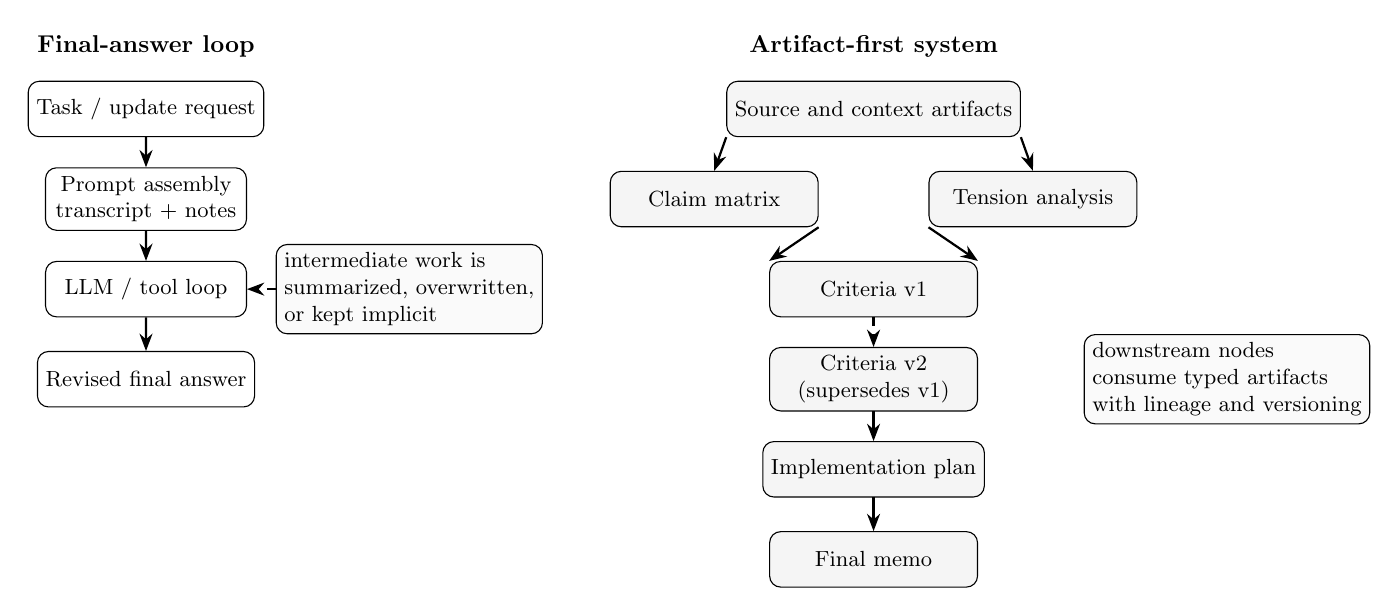
\begin{tikzpicture}[
  font=\small,
  scale=0.88,
  transform shape,
  node distance=7mm and 10mm,
  box/.style={draw, rounded corners, align=center, minimum width=29mm, minimum height=8mm},
  artifact/.style={draw, rounded corners, align=center, minimum width=30mm, minimum height=8mm, fill=black!4},
  state/.style={draw, rounded corners, align=left, minimum width=34mm, minimum height=8mm, fill=black!2},
  arrow/.style={-{Stealth[length=2.2mm]}, thick},
  dashedarrow/.style={-{Stealth[length=2.2mm]}, dashed, thick}
]
\node[font=\bfseries] at (0,0) {Final-answer loop};
\node[box] (goal) at (0,-0.9) {Task / update request};
\node[box] (transcript) at (0,-2.2) {Prompt assembly\\transcript + notes};
\node[box] (loop) at (0,-3.5) {LLM / tool loop};
\node[box] (answer) at (0,-4.8) {Revised final answer};
\node[state] (hidden) at (3.8,-3.5) {intermediate work is\\summarized, overwritten,\\or kept implicit};
\draw[arrow] (goal) -- (transcript);
\draw[arrow] (transcript) -- (loop);
\draw[arrow] (loop) -- (answer);
\draw[dashedarrow] (hidden.west) -- (loop.east);

\node[font=\bfseries] at (10.5,0) {Artifact-first system};
\node[artifact] (src) at (10.5,-0.9) {Source and context artifacts};
\node[artifact] (claims) at (8.2,-2.2) {Claim matrix};
\node[artifact] (tensions) at (12.8,-2.2) {Tension analysis};
\node[artifact] (criteria1) at (10.5,-3.5) {Criteria v1};
\node[artifact] (criteria2) at (10.5,-4.8) {Criteria v2\\(supersedes v1)};
\node[artifact] (plan) at (10.5,-6.1) {Implementation plan};
\node[artifact] (memo) at (10.5,-7.4) {Final memo};
\draw[arrow] (src.south west) -- (claims.north);
\draw[arrow] (src.south east) -- (tensions.north);
\draw[arrow] (claims.south east) -- (criteria1.north west);
\draw[arrow] (tensions.south west) -- (criteria1.north east);
\draw[dashedarrow] (criteria1.south) -- (criteria2.north);
\draw[arrow] (criteria2.south) -- (plan.north);
\draw[arrow] (plan.south) -- (memo.north);
\node[state] at (15.6,-4.8) {downstream nodes\\consume typed artifacts\\with lineage and versioning};
\end{tikzpicture}

\end{document}